\aufgabe{}{

You receive a dataset with 1000 data points from a data generating process with $X_1 \sim \mathcal{U}(-1, 1)$, $X_2 = X_1^2  + \delta$, $\delta \sim \mathcal{N}(0,0.04)$ and $Y = 5 X_1 - 2X_2 + \epsilon, \epsilon \sim \mathcal{N}(0,1)$. 

The fitted linear model has the following form: 
$\fh(\xv) = \hat \beta_0 + \hat\beta_1 \xv_1 + \hat\beta_2 \xv_2 + \hat\beta_3 \xv_1 \xv_2$.

Below, the PDP (first row) and ALE (second row) for $x_1$ and $x_2$ are shown. 
\begin{enumerate}
\item Interprete the plots with respect to the feature effect of $x_1$ and $x_2$. 
\item Would you rather trust the PDP or ALE plot? Give reasons for your 
decision. 
\end{enumerate}

\begin{center}
  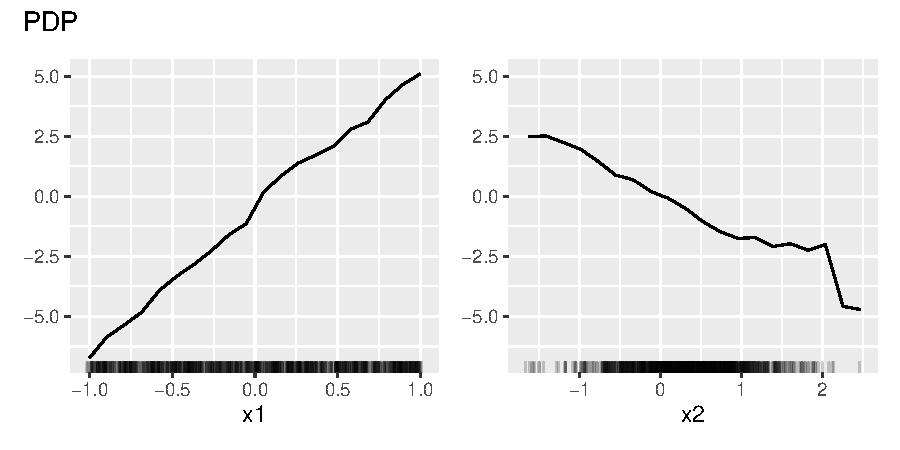
\includegraphics[width=\maxwidth]{figure/PDP_Plot.pdf}
\end{center}


\begin{center}
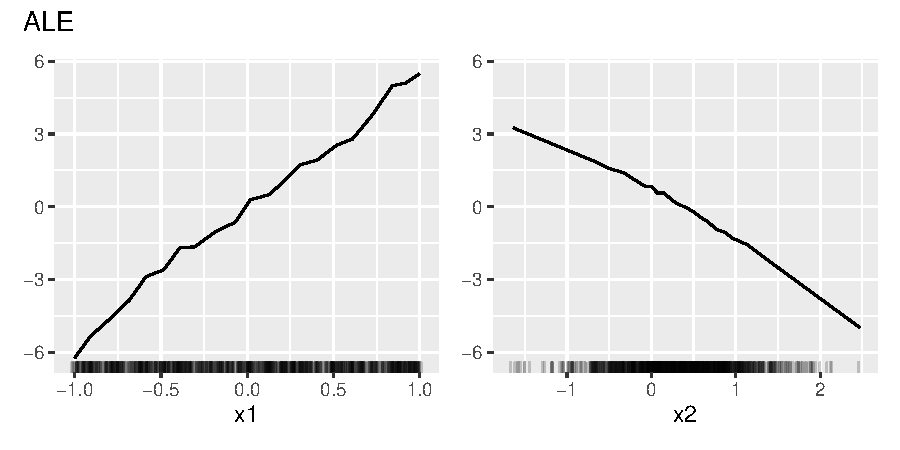
\includegraphics[width=\maxwidth]{figure/ALE_Plot.pdf}
\end{center}


}
